% Neutral draft layout. The journal is not chosen yet (open item); replace this file with the journal module's main.tex.
\documentclass[11pt]{article}
\usepackage[T1]{fontenc}
\usepackage{lmodern}
\usepackage[utf8]{inputenc}
\usepackage[margin=2.5cm]{geometry}
\usepackage{graphicx,amsmath,booktabs}
\DeclareGraphicsExtensions{.pdf,.png}
% Generated by pipeline_v2/make_macros.py from pipeline_v2/results; do not edit by hand.
\newcommand{\NSegments}{24}
\newcommand{\NStarsRun}{23}
\newcommand{\NNotRun}{4}
\newcommand{\NLow}{23}
\newcommand{\NSunYears}{51}
\newcommand{\NSurr}{1000}
\newcommand{\SeedBase}{20261124}
\newcommand{\NConfigs}{4}
\newcommand{\NFracs}{5}
\newcommand{\LMin}{28}
\newcommand{\LMax}{36}
\newcommand{\HOneNMinOne}{44}
\newcommand{\HOneMeanMinOne}{0.1810}
\newcommand{\HOneRawMinOne}{0.0035}
\newcommand{\HOneSigAMinOne}{0.0027}
\newcommand{\HOneSigBMinOne}{0.0028}
\newcommand{\HOneNMinTwo}{315}
\newcommand{\HOneMeanMinTwo}{0.1724}
\newcommand{\HOneRawMinTwo}{0.0058}
\newcommand{\HOneSigAMinTwo}{0.0054}
\newcommand{\HOneSigBMinTwo}{0.0048}
\newcommand{\HOneNGrand}{103}
\newcommand{\HOneMeanGrand}{0.1705}
\newcommand{\HOneRawGrand}{0.0020}
\newcommand{\HOneSigAGrand}{0.0019}
\newcommand{\HOneSigBGrand}{0.0015}
\newcommand{\HOnePRaw}{$9\times10^{-6}$}
\newcommand{\HOnePCorrA}{$9\times10^{-3}$}
\newcommand{\HOnePCorrB}{$1\times10^{-6}$}
\newcommand{\HOneFRaw}{2.95}
\newcommand{\HOneFCorrA}{1.90}
\newcommand{\NCellsHalf}{192}
\newcommand{\NSigHalf}{2}
\newcommand{\MaxConcAR}{1}
\newcommand{\NConcThreeAR}{0}
\newcommand{\NTauPosARSOne}{11}
\newcommand{\MaxConcVar}{0}
\newcommand{\NConcThreeVar}{0}
\newcommand{\NTauPosVarSOne}{12}
\newcommand{\MaxConcSweep}{4}
\newcommand{\HOnePTwoBound}{$<10^{-3}$}
\newcommand{\NCatalog}{112}
\newcommand{\NBaumStars}{59}
\newcommand{\NVTwoStars}{35}
\newcommand{\HDHTauNone}{0.40}
\newcommand{\HDHPNone}{0.28}
\newcommand{\HDHTauSOne}{0.55}
\newcommand{\HDHPSOne}{0.20}
\newcommand{\SunTauNone}{0.26}
\newcommand{\SunPNone}{0.32}
\newcommand{\SunTauSOne}{0.25}
\newcommand{\SunPSOne}{0.27}
\newcommand{\HDHL}{30}
\newcommand{\HDHVarTauSOne}{\textminus{}0.75}
\newcommand{\HDHVarPSOne}{0.91}
\newcommand{\HDHVarTauNone}{0.08}
\newcommand{\HDHVarPNone}{0.47}
\newcommand{\WinHD}{15}
\newcommand{\WinSun}{26}
\newcommand{\NFigTests}{48}
\newcommand{\MedACNone}{0.58}
\newcommand{\MedACSOne}{\textminus{}0.31}
\newcommand{\NACNoneHigh}{15}
\newcommand{\NStarsMetric}{23}
\newcommand{\RHKMaxDiff}{0}
\newcommand{\RHKNCompare}{960}
\newcommand{\PrimN}{11}
\newcommand{\PrimNFlat}{4}
\newcommand{\PrimP}{0.89}
\newcommand{\PrimU}{13}
\newcommand{\PrimMedVL}{\textminus{}0.37}
\newcommand{\PrimMedFlat}{\textminus{}0.29}
\newcommand{\NHolmTests}{30}
\newcommand{\NHolmSig}{2}
\newcommand{\NRawSig}{3}
\newcommand{\CycFlatPSOne}{0.0020}
\newcommand{\CycFlatHolmSOne}{0.0101}
\newcommand{\CycFlatPNone}{0.0081}
\newcommand{\CycFlatHolmNone}{0.0404}
\newcommand{\AutoUp}{3.2}
\newcommand{\AutoLo}{4.2}
\newcommand{\RHKMaxPDiff}{0.39}
\newcommand{\NSigHalfRHK}{3}
\newcommand{\NHolmSigThirty}{0}
\newcommand{\CycFlatHolmThirtySOne}{0.06}
\newcommand{\CycFlatHolmThirtyNone}{0.23}
\newcommand{\MinPCycleFlat}{0.0020}
\newcommand{\MinPFourFour}{0.014}
\newcommand{\ResAmpTen}{18}
\newcommand{\ResAmpTwelve}{13}
\newcommand{\ResAmpSixteen}{7}
\newcommand{\NGroupFlat}{4}
\newcommand{\NGroupCycle}{8}
\newcommand{\NGroupVar}{7}
\newcommand{\NGroupLong}{4}
\newcommand{\AUCTwentyFour}{0.59}
\newcommand{\AUCThirty}{0.60}
\newcommand{\AUCForty}{0.63}

% Design constants quoted in the text (not results). Origin of each value in the project record:
\newcommand{\NoiseMW}{1.2}      % instrumental noise, Mount Wilson, percent of mean S (Luhn et al. 2022, Sect. 3.1; decision D45)
\newcommand{\NoiseKeck}{0.3}    % same, Keck (same source; quoted as an upper limit)
\newcommand{\MinSeg}{24}        % minimum segment, years (decisions D99, D100)
\newcommand{\LowMax}{39}        % upper end of the "low precision" band, years (D100)
\newcommand{\AdeqMin}{40}       % start of the "adequate" band, years (D100)
\newcommand{\SizeLo}{3}         % accepted range of the size check, percent, fixed before the run
\newcommand{\SizeHi}{7}

\title{Critical slowing down near stellar activity minima: a test on Mount Wilson S-index series}
\author{Draft; author block to be completed by the author}
\date{}
\begin{document}
\maketitle
\begin{abstract}
Some Sun-like stars lose their activity cycle, as the Sun did in the Maunder minimum. If such a loss behaves like a critical transition, the lag-1 autocorrelation and the variance of the activity record should rise beforehand. We test this on annual means of the Mount Wilson Ca\,\textsc{ii} H and K index (S) for \NStarsRun{} stars and for a composite solar record, in segments of \LMin{} to \NSunYears{} years. Rolling-window indicators are computed for the original series and three detrended versions, and tested against \NSurr{} ARMA surrogates that reproduce the gaps and interpolation of the data. HD~166620, a candidate for entering a grand minimum, has lower S-index variability in the minimum than in two earlier cycle minima (H1, confirmatory, using intervals already published). No segment shows a consistent rise in the temporal indicators (H2). The Mount Wilson record of HD~166620 ends before its transition, so H2 could not be tested as designed, and the other segments are a null scan of series with no known transition. The surrogate test has nominal size (\AutoUp\,\% and \AutoLo\,\% at a nominal 5\,\%) but little power at these lengths. Two group differences in normalized variance survive Holm correction within blocks, but not over all tests; we attribute them to cycle amplitude, which we did not test.
\end{abstract}
\section{Introduction}

Stars of roughly solar type show chromospheric activity that is cyclic in some, irregular in others and nearly constant in a few \cite{baliunas1995}. The Sun itself went through the Maunder minimum, when the cycle was strongly suppressed \cite{usoskin2017}. Whether a star that is about to lose its cycle gives a warning is the question we take up here. The idea comes from dynamical systems: near a transition where a stable state disappears, the recovery from small perturbations slows down, and that shows up as a rising lag-1 autocorrelation and rising variance in the time series \cite{scheffer2009,held2004}. Rolling-window indicators of this kind, with significance tested against surrogate series, are the standard recipe \cite{dakos2012}.

Two data sets make a test possible. The Mount Wilson HK Project followed dozens of stars for decades, and Baum et al.\ \cite{baum2022} assembled the series of 59 stars from Mount Wilson and Keck with instrument labels. Luhn et al.\ \cite{luhn2022} showed that HD~166620 went from a cyclic state to a grand minimum, which gives one star with states on both sides of the transition. The Sun has its own calibrated S-index record \cite{egeland2017}.

We ask two questions, declared before any indicator was computed on a real star. H1 (confirmatory) compares the S-index variability of HD~166620 across its three states. H2 (exploratory, one star) asks whether the rolling indicators of HD~166620 rise before the grand minimum. The temporal indicators are also computed in every other star with a long enough Mount Wilson segment; those results are descriptive, and the sample is too small to carry a group comparison on its own.

\section{Data and methods}

\subsection{Sample and series}

The catalogue is the frozen version of Table~2 of Baliunas et al.\ \cite{baliunas1995} (\NCatalog{} stars), whose classes are Flat (S-index scatter below about 1--1.5\,\% of the mean), Cycle (a cycle period with a false-alarm class; we use the ``excellent'' ones), Var (variable without a periodic signal) and Long (variability on timescales longer than 25 years). Series come from three sources: the \NBaumStars{} stars of Baum et al.\ \cite{baum2022} (Table~1; points flagged as outliers are removed, points flagged both as one-day and outlier are kept), the \NVTwoStars{} stars of the HK Project v2001 files, and the calibrated solar S index of Egeland et al.\ \cite{egeland2017} (Table~4, 1966--2016, a composite of several instruments). Calibration stars, two binaries and stars with no series in any source were excluded before any indicator was computed. Our binarity rule leaves five clean Flat stars, of which four have a series. The stars analyzed are \NGroupFlat{} Flat, \NGroupCycle{} Cycle, \NGroupVar{} Var and \NGroupLong{} Long, plus the Sun, which is treated as exploratory.

For the temporal indicators each star is reduced to annual means of S, the mean of all observations in a calendar year. Only the Mount Wilson era is used, so no segment crosses the change to Keck; the change between the two Mount Wilson photometers inside that era is not corrected, and the solar composite combines five instruments as calibrated by Egeland et al. Gaps of one or two missing years are filled by linear interpolation and the filled points are marked; gaps of three or more years split the series into segments. Indicators are computed only in segments of at least \MinSeg{} years, so that a window of 50\,\% has at least 12 points and 13 windows. Segments of \MinSeg--\LowMax{} years are labeled low precision and their results exploratory; segments of \AdeqMin{} years or more are labeled adequate. \NStarsRun{} stars have such a segment (\LMin--\LMax{} years) and so does the Sun (\NSunYears{} years); \NNotRun{} further stars have a Mount Wilson segment shorter than \MinSeg{} years and receive a description only.

\subsection{Indicators and detrending}

In each segment we compute the lag-1 autocorrelation (AR(1) coefficient) and the variance in a sliding window, and the Kendall $\tau$ of each against window index (no tie correction; the same computation is used for the data and the surrogates). The window is a fraction $f$ of the segment length $L$, $w = \mathrm{round}(fL)$, with $f = 0.25$, 0.375, 0.5, 0.625 and 0.75; $f = 0.5$ is the default. The series is analyzed in four configurations: the original series, and the residual of a Gaussian smooth with $\sigma = 1$, 3 or 5 years (edges handled by repeating the end values). A Gaussian smooth of width $\sigma$ keeps a fraction $\exp[-\tfrac{1}{2}(2\pi\sigma/P)^2]$ of the amplitude of a cycle of period $P$; the residual is thus a high-pass version of the series, not the series without its cycle. A segment is flagged for an indicator when $\tau > 0$ with $p < 0.05$ in at least three of the four configurations. H2 requires this for both indicators.

\subsection{Significance}

The $p$ value of each $\tau$ comes from \NSurr{} surrogate series from an ARMA($p,q$) model with $p,q \le 2$ chosen by AIC, fitted by maximum likelihood to the series (or residual) being tested, with Gaussian innovations and a burn-in of 100 steps. Each surrogate receives the same gap positions and the same linear interpolation as the data. We report $p = P(\tau^{*} \ge \tau)$, where $\tau^{*}$ is the surrogate statistic, with the correction $(k+1)/(N+1)$ for $k$ exceedances in $N$ surrogates; this is the tail in the direction of critical slowing down. The size of the procedure was checked on synthetic AR(1) series with no trend (600 series of 30 years, three interpolated points, coefficient 0.5), with the acceptance range of \SizeLo--\SizeHi\,\% for a nominal 5\,\% fixed beforehand. Power was examined in an earlier simulation, before any stellar series was analyzed, in which the AR(1) coefficient either stayed at 0.5 or rose linearly from 0.3 to 0.7 (600 series per length, window 50\,\%, no cycle); the quantity reported is the area under the ROC curve (AUC) of $\tau$ for trend against null.

\subsection{State comparison for HD~166620}

For H1 we use the raw (not annual) series of Luhn et al.\ \cite{luhn2022}, in the three states they define: minimum~1 (1971--1975), minimum~2 (1987--1991) and the grand minimum (from 2004). The variability $\sigma_S$ of a state is the standard deviation of the interval with the instrumental noise variance removed in quadrature, the noise being \NoiseMW\,\% of the mean S for Mount Wilson and \NoiseKeck\,\% for Keck as quoted by Luhn et al.\ (method A, primary). As a sensitivity check, method B takes the mean over seasons of the same corrected value. Variances are compared with a two-sided $F$ test, with raw and with corrected values; the test treats observations as independent, which they are not (Sect.~\ref{sec:disc}).

\subsection{R$'_{\rm HK}$}

S is also converted to $R'_{\rm HK}$ with the recipe and color correction of Noyes et al.\ \cite{noyes1984}, using $B\!-\!V$ from the California Legacy Survey V catalogue \cite{isaacson2024} when the star is in it and from Baliunas et al.\ otherwise. The photospheric term of that calibration is valid for $0.44 < B\!-\!V < 0.82$; stars outside are marked in Table~\ref{tab:seg}. For a given $B\!-\!V$ the conversion is linear in S, so $\tau$ is unchanged and the run serves as a check.

\subsection{Group comparisons}

Groups are compared per star with the lag-1 autocorrelation and the normalized variance of the longest segment. The primary pair is Var and Long together against Flat, lag-1 autocorrelation of the $\sigma = 1$ residual, one-sided Mann--Whitney test, fixed before the tests were read. The remaining pairs (five per metric and configuration) are corrected with the Holm procedure within each metric and configuration block; Holm over all 30 tests is also reported (see below). The groups have four to eight stars, so the smallest attainable one-sided $p$ is \MinPCycleFlat{} (eight against four) or \MinPFourFour{} (four against four).

\subsection{Analysis log}

Fixed before the stellar run: the sample and groups, the segment rule, windows, detrending, surrogate design, H1 and H2, and the size check with its acceptance range. Decided after the run, without changing any computed value: the tail of $p$ (upper tail; the lower tail is also computed); keeping the points flagged both as one-day and outlier, which affects two stars (HD~190360 and HD~217014; with the opposite choice HD~190360 would fall below the minimum length); and the family of the Holm correction (blocks of five instead of all 30 tests). Both Holm families are reported.

\subsection{Software}

Python with NumPy, pandas, SciPy and statsmodels; the pipeline, the seeds (base \SeedBase) and the single official run are in the repository.

\section{Results}

\subsection{Size and power of the surrogate test}

On synthetic AR(1) series with no trend, the test rejected at the 5\,\% level in \AutoUp\,\% of the series with the upper-tail $p$ and in \AutoLo\,\% with the lower-tail $p$, inside the accepted range; it is slightly conservative. In the earlier power simulation, the AUC of $\tau$ for a rising coefficient against a constant one was \AUCTwentyFour{} for segments of 24 years, \AUCThirty{} for 30 and \AUCForty{} for 40 (1 would be perfect discrimination, 0.5 none). At the lengths used here the indicator therefore separates a rising autocorrelation from a stationary one only weakly, even without a cycle in the series.

\subsection{H1: variability of HD~166620 by state}

Table~\ref{tab:h1} gives the three states. The mean S is lower in the grand minimum (\HOneMeanGrand) than in minimum~1 (\HOneMeanMinOne), a difference we did not test. The variability $\sigma_S$ (method A) falls from \HOneSigAMinOne{} in minimum~1 to \HOneSigAGrand{} in the grand minimum; minimum~2 has the largest value, \HOneSigAMinTwo{} (Fig.~\ref{fig:h1}). Method B gives the same ordering (\HOneSigBMinOne, \HOneSigBMinTwo, \HOneSigBGrand). The $F$ test of minimum~1 against the grand minimum gives $p = $ \HOnePRaw{} with the raw variances and $p = $ \HOnePCorrA{} with the corrected ones (method A), and $p = $ \HOnePCorrB{} with method B; minimum~2 against the grand minimum gives \HOnePTwoBound{} in every version. The $p$ values are reported to one significant figure because the test treats clustered, autocorrelated observations as independent.

\begin{table}[h]
\centering
\begin{tabular}{lrrrrr}
\hline
State & $N$ & $\langle S\rangle$ & raw $\sigma$ & $\sigma_S$ (A) & $\sigma_S$ (B) \\
\hline
Minimum 1 (1971--75) & \HOneNMinOne & \HOneMeanMinOne & \HOneRawMinOne & \HOneSigAMinOne & \HOneSigBMinOne \\
Minimum 2 (1987--91) & \HOneNMinTwo & \HOneMeanMinTwo & \HOneRawMinTwo & \HOneSigAMinTwo & \HOneSigBMinTwo \\
Grand minimum (2004--) & \HOneNGrand & \HOneMeanGrand & \HOneRawGrand & \HOneSigAGrand & \HOneSigBGrand \\
\hline
\end{tabular}
\caption{HD~166620 by state: number of observations, mean S, raw standard deviation of the interval, and $\sigma_S$ with the instrumental noise removed in quadrature, methods A and B.}
\label{tab:h1}
\end{table}

\subsection{Temporal indicators}
\label{sec:temporal}

\begin{table}[p]
\centering\small
\begin{tabular}{llrrrrrrrrr}
\hline
HD & Group & Years & $L$ & Interp. & $B\!-\!V$ & $\tau$ & $p$ & $\tau$ & $p$ & Conc. \\
 & & & & & & \multicolumn{2}{c}{no removal} & \multicolumn{2}{c}{$\sigma = 1$ yr} & AR/Var \\
\hline
10700 & Flat & 1967--1995 & 29 & 0 & 0.66 & -0.10 & 0.566 & -0.57 & 0.852 & 0/0 \\
23249 & Flat & 1967--1995 & 29 & 0 & 0.88 & +0.75 & 0.032 & +0.38 & 0.268 & 1/0 \\
182572 & Flat & 1967--2001 & 35 & 10 & 0.73 & -0.40 & 0.766 & -0.58 & 0.577 & 0/0 \\
190360 & Flat & 1967--1994 & 28 & 5 & 0.72 & -0.83 & 0.988 & -0.35 & 0.297 & 0/0 \\
Sun & Cycle & 1966--2016 & 51 & 2 & 0.66 & +0.26 & 0.321 & +0.25 & 0.272 & 0/0 \\
4628 & Cycle & 1966--1995 & 30 & 0 & 0.85 & +0.57 & 0.102 & +0.33 & 0.369 & 0/0 \\
10476 & Cycle & 1966--2001 & 36 & 0 & 0.80 & +0.13 & 0.396 & -0.35 & 0.712 & 0/0 \\
26965 & Cycle & 1967--1995 & 29 & 0 & 0.76 & +0.50 & 0.157 & +0.42 & 0.246 & 0/0 \\
103095 & Cycle & 1968--2001 & 34 & 0 & 0.67 & -0.44 & 0.796 & -0.69 & 0.925 & 0/0 \\
152391 & Cycle & 1966--2001 & 36 & 0 & 0.72 & -0.47 & 0.814 & +0.44 & 0.253 & 0/0 \\
160346 & Cycle & 1966--2001 & 36 & 0 & 0.96 & -0.11 & 0.606 & -0.26 & 0.667 & 0/0 \\
166620 & Cycle & 1966--1995 & 30 & 0 & 0.83 & +0.40 & 0.276 & +0.55 & 0.197 & 0/0 \\
201091 & Cycle & 1967--2001 & 35 & 0 & 1.15 & -0.05 & 0.537 & +0.24 & 0.391 & 0/0 \\
3795 & Var & 1966--1994 & 29 & 1 & 0.68 & -0.20 & 0.628 & -0.18 & 0.604 & 0/0 \\
39587 & Var & 1966--2001 & 36 & 0 & 0.59 & -0.23 & 0.653 & -0.29 & 0.648 & 0/0 \\
75332 & Var & 1966--2001 & 36 & 0 & 0.49 & -0.43 & 0.745 & -0.10 & 0.561 & 0/0 \\
101501 & Var & 1968--1995 & 28 & 0 & 0.70 & +0.71 & 0.065 & +0.35 & 0.278 & 0/0 \\
115383 & Var & 1966--2001 & 36 & 0 & 0.58 & +0.26 & 0.323 & -0.05 & 0.544 & 0/0 \\
131156A & Var & 1967--2001 & 35 & 0 & 0.76 & +0.15 & 0.413 & +0.05 & 0.495 & 0/0 \\
217014 & Var & 1966--1995 & 30 & 4 & 0.65 & +0.07 & 0.225 & +0.18 & 0.026 & 1/0 \\
25998 & Long & 1966--2001 & 36 & 0 & 0.46 & -0.60 & 0.905 & +0.33 & 0.298 & 0/0 \\
35296 & Long & 1966--2001 & 36 & 0 & 0.53 & -0.73 & 0.975 & -0.70 & 0.933 & 0/0 \\
141004 & Long & 1966--1995 & 30 & 1 & 0.59 & +0.70 & 0.064 & -0.37 & 0.696 & 0/0 \\
176095 & Long & 1966--2001 & 36 & 1 & 0.46 & -0.24 & 0.564 & -0.33 & 0.522 & 0/0 \\
\hline
\end{tabular}

\caption{Segments with an indicator. $L$: length in years; Interp.: interpolated years; $\tau$ and $p$: Kendall $\tau$ of the rolling lag-1 autocorrelation (window 50\,\%) and its surrogate $p$, for the original series and for the $\sigma = 1$ year residual; Conc.: number of the four configurations with $\tau > 0$ and $p < 0.05$, for the lag-1 autocorrelation and for the variance (the other two configurations are not shown). $^{a}$ $B\!-\!V$ outside 0.44--0.82. $^{b}$ Composite of several instruments; exploratory.}
\label{tab:seg}
\end{table}

Table~\ref{tab:seg} lists the \NSegments{} segments. With a window of 50\,\%, \NSigHalf{} of the \NCellsHalf{} combinations of segment, indicator and configuration have $\tau > 0$ and $p < 0.05$: HD~23249 for the original series ($\tau = +0.75$, $p = 0.032$) and HD~217014 for the $\sigma = 1$ residual ($\tau = +0.18$, $p = 0.026$), both for the lag-1 autocorrelation. No segment reaches three of four configurations for the lag-1 autocorrelation (maximum \MaxConcAR) or for the variance (maximum \MaxConcVar). Across all five window lengths, the largest number of concordant configurations in one segment is \MaxConcSweep{} of 20; we computed no null reference for this count.

For HD~166620 ($L = $ \HDHL{} years, Mount Wilson era, which ends before the transition) the window is \WinHD{} years. The lag-1 autocorrelation has $\tau = $ \HDHTauNone{} ($p = $ \HDHPNone) for the original series and $\tau = $ \HDHTauSOne{} ($p = $ \HDHPSOne) for the $\sigma = 1$ residual (Fig.~\ref{fig:roll}); the variance has $\tau = $ \HDHVarTauNone{} ($p = $ \HDHVarPNone) and $\tau = $ \HDHVarTauSOne{} ($p = $ \HDHVarPSOne). For the Sun (window \WinSun{} years) the lag-1 autocorrelation has $\tau = $ \SunTauNone{} ($p = $ \SunPNone) and $\tau = $ \SunTauSOne{} ($p = $ \SunPSOne).

Over the \NSegments{} segments, $\tau$ of the lag-1 autocorrelation is positive for the $\sigma = 1$ residual in \NTauPosARSOne{} and $\tau$ of the variance in \NTauPosVarSOne{} (Fig.~\ref{fig:tau}). Across the \NStarsMetric{} stars, the lag-1 autocorrelation of the whole longest segment has a median of \MedACNone{} for the original series (above 0.5 in \NACNoneHigh{} stars) and \MedACSOne{} for the $\sigma = 1$ residual.

Converting S to $R'_{\rm HK}$ leaves $\tau$ unchanged in all \RHKNCompare{} comparisons (largest difference \RHKMaxDiff). The surrogate $p$ values do not carry over as closely: for the same segment and configuration at a window of 50\,\%, the $p$ of the two runs differ by up to \RHKMaxPDiff{}, and \NSigHalfRHK{} cells instead of \NSigHalf{} fall below 0.05. Each run fits its own ARMA model and draws its own surrogates, so this spread measures how unstable the fit is on 28 to 36 points.

\subsection{Group comparisons}

The primary pair (Var and Long against Flat, $\sigma = 1$ residual) has $n = \PrimN$ and \PrimNFlat{} stars, $U = \PrimU$, $p = \PrimP$; the medians of the lag-1 autocorrelation are \PrimMedVL{} and \PrimMedFlat. Of the \NHolmTests{} remaining tests, \NRawSig{} have an uncorrected $p < 0.05$. With Holm within blocks, \NHolmSig{} remain below 0.05, both Cycle against Flat in the normalized variance: with $\sigma = 1$, $p = $ \CycFlatPSOne{} and $p_{\rm Holm} = $ \CycFlatHolmSOne; for the original series, $p = $ \CycFlatPNone{} and $p_{\rm Holm} = $ \CycFlatHolmNone. With Holm over all \NHolmTests{} tests, \NHolmSigThirty{} remain (the same two comparisons give \CycFlatHolmThirtySOne{} and \CycFlatHolmThirtyNone).

\begin{figure}[h]
\centering
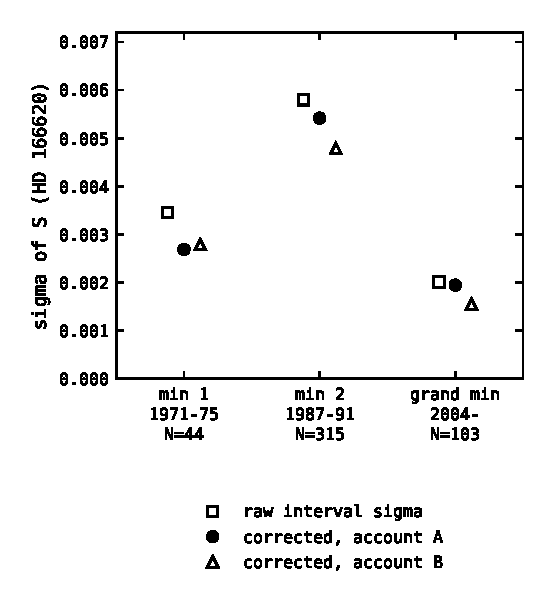
\includegraphics[width=0.6\textwidth]{figures/figure1}
\caption{Variability $\sigma$ of the S index of HD~166620 in three states (data of Luhn et al.). $N$ is the number of observations in the interval. Squares: standard deviation of the whole interval (raw). Circles (method A): interval standard deviation with the instrumental noise variance removed in quadrature. Triangles (method B): mean over seasons of the same corrected value. No uncertainties are shown; the corresponding $F$ tests are in the text.}
\label{fig:h1}
\end{figure}
\begin{figure}[h]
\centering
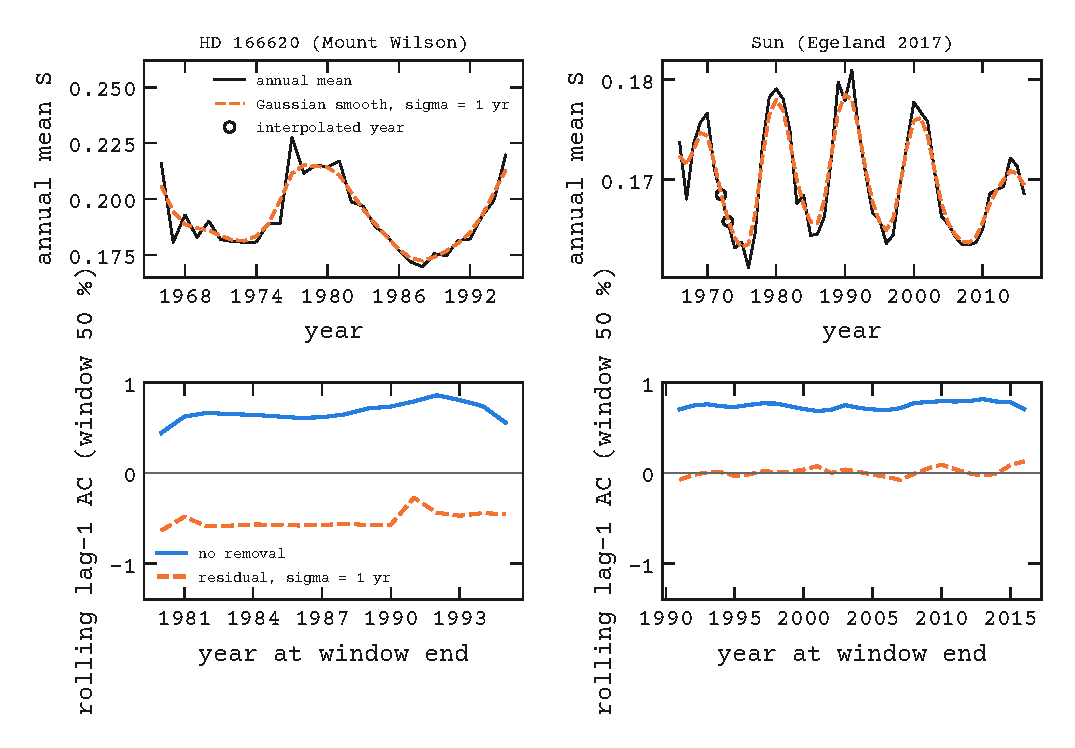
\includegraphics[width=\textwidth]{figures/figure2}
\caption{Top: annual mean S (solid) and its Gaussian smooth with $\sigma = 1$ year (dashed) for HD~166620 (Mount Wilson era) and the Sun (composite series of Egeland et al.; exploratory). Open circles mark interpolated years: none for HD~166620, two for the Sun. The two panels have different vertical ranges. Bottom: rolling lag-1 autocorrelation in a window of 50\,\% of the segment (\WinHD{} years for HD~166620, \WinSun{} for the Sun), plotted at the end year of each window, for the original series (solid) and for the residual, that is, the series minus its smooth (dashed). The horizontal axes share one scale in years.}
\label{fig:roll}
\end{figure}
\begin{figure}[h]
\centering
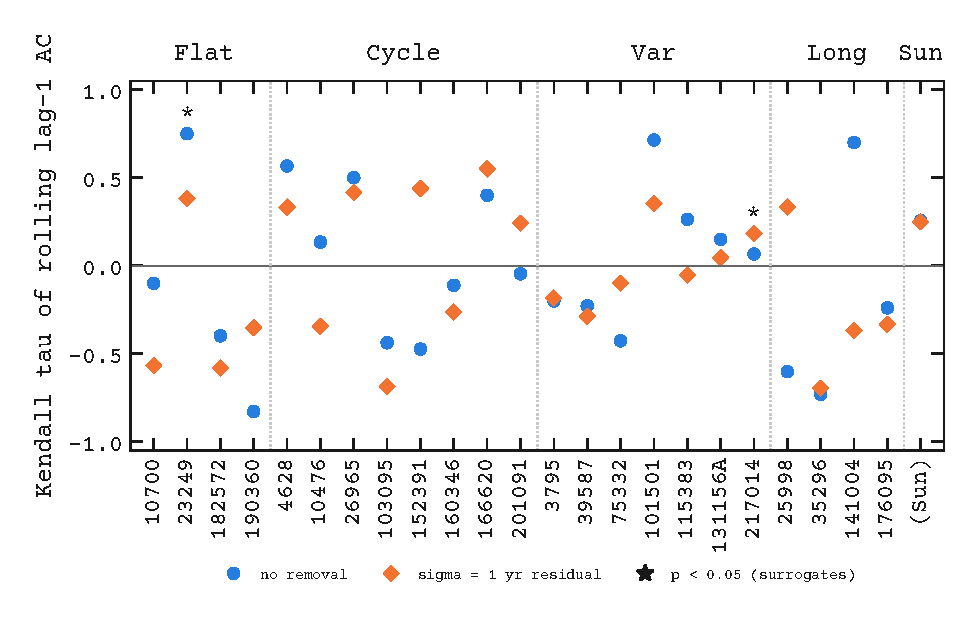
\includegraphics[width=\textwidth]{figures/figure3}
\caption{Kendall $\tau$ of the rolling lag-1 autocorrelation (window of 50\,\% of the longest Mount Wilson segment of each star, annual mean S) for the original series (circles) and the $\sigma = 1$ year residual (diamonds). Stars are grouped as Flat, Cycle, Var and Long and sorted by HD number within a group, which carries no meaning; the Sun (composite series, exploratory) is shown last. An asterisk above a marker means $p < 0.05$ for that configuration, with $p = P(\tau^{*} \ge \tau)$ against the ARMA surrogates (one-sided, upper tail, not corrected for the \NFigTests{} tests shown). The Sun's two markers nearly coincide.}
\label{fig:tau}
\end{figure}

\section{Discussion}
\label{sec:disc}

\paragraph{State comparison.} H1 asked whether the S-index variability of HD~166620 in the grand minimum is smaller than in the cycle minima. It is, by both methods and for both minima (Table~\ref{tab:h1}). We treat this as descriptive. It rests on one star, on single intervals, and on an $F$ test whose $p$ values are not credible at face value: the observations inside a season are strongly correlated (minimum~2 has \HOneNMinTwo{} points in four seasons), and the correction subtracts a fixed fraction of the mean as instrumental noise, with a different fraction for the instrument that observed the grand minimum. A lower variance in a lower-activity state is also what one expects without any dynamical transition. The direction of the difference is the finding; its significance is not.

\paragraph{Temporal indicators.} H2 was not supported: for HD~166620 the variance has $\tau \le 0$ for the $\sigma = 1$ residual and for the larger smoothing widths, and the lag-1 autocorrelation has $p \ge 0.05$ in all four configurations. But the test was not possible as designed. The Mount Wilson record of HD~166620 ends in 1995, before the transition, and we could not find the original Mount Wilson observations for 1995--2002 in a public source, so the approach to the grand minimum is not sampled. The other \NSegments{} segments are series with no known transition; they form a null scan, and the absence of a flagged segment is the expected outcome when nothing is there to find. A decisive test needs an annual or finer series that runs through a transition.

\paragraph{Power.} The surrogate test has nominal size, slightly conservative (\AutoUp\,\% at a nominal 5\,\%), and in 192 combinations it flagged two where about ten would be expected by chance if the combinations were independent, which they are not. Its power is low: AUC of \AUCTwentyFour{} to \AUCForty{} for a rising autocorrelation without any cycle, at 24 to 40 years. With a deterministic cycle present, an ARMA model fitted to the series can absorb part of it, so the surrogate null then mimics the cycle and the test is less able to react to changes in it. We did not quantify this. A null outcome here is therefore weak evidence against critical slowing down before a loss of cycle, and the instability of the ARMA fit on short segments (Sect.~\ref{sec:temporal}) adds to that.

\paragraph{What the indicators measure.} A Gaussian smooth of width one year keeps most of a cycle of ten to sixteen years, so the $\sigma = 1$ residual keeps only \ResAmpTen, \ResAmpTwelve{} and \ResAmpSixteen\,\% of the amplitude of cycles of 10, 12 and 16 years. This explains the negative median lag-1 autocorrelation of the residual (\MedACSOne) against \MedACNone{} for the original series. Windows of 12 to 26 points cover about one cycle, so the rolling indicators follow cycle phase more than recovery rate, and the four configurations are not four independent views of the noise. The normalized variance differs between Cycle and Flat stars without any critical slowing down, through the cycle amplitude alone. We attribute the two comparisons that survive within-block Holm correction to this, as an interpretation we did not test; they do not survive Holm over all tests.

\paragraph{Limits.} Segments with interpolated years (up to ten in one star), stars outside the validity range of the $R'_{\rm HK}$ calibration, and the composite character of the solar series are marked in Table~\ref{tab:seg}; we ran no sensitivity check on the interpolation. The Sun is the only segment labeled adequate, but its level can shift where instruments change. Group sizes (four to eight) make every group test low in power, and stars entered through the availability of a series, so the groups are convenience samples. A repeat of the analysis on a series that crosses a known transition, with a power curve at the real segment lengths and with a cycle in the injected series, is the next step.

\section{Conclusions}

The S-index variability of HD~166620 in its grand minimum is lower than in both cycle minima. Rolling lag-1 autocorrelation and variance, computed on annual Mount Wilson series of \LMin{} to \NSunYears{} years in \NSegments{} segments, show no consistent rise: no segment is flagged in three of four detrending configurations, and the test has low power. The group differences that survive correction are the cycle amplitude.

% Author's declarations (conflicts of interest, funding, data and code availability, acknowledgements, AI-use statement):
% to be written by the author. Data and code: the repository with the pipeline and the results.
\section*{Data availability}
Series are from the public sources cited in the Methods; the processed results and the code are in the project repository (link to be added at publication).

\bibliographystyle{plain}
\bibliography{references}
\end{document}
